\documentclass[man]{apa6}
\usepackage{lmodern}
\usepackage{amssymb,amsmath}
\usepackage{ifxetex,ifluatex}
\usepackage{fixltx2e} % provides \textsubscript
\ifnum 0\ifxetex 1\fi\ifluatex 1\fi=0 % if pdftex
  \usepackage[T1]{fontenc}
  \usepackage[utf8]{inputenc}
\else % if luatex or xelatex
  \ifxetex
    \usepackage{mathspec}
  \else
    \usepackage{fontspec}
  \fi
  \defaultfontfeatures{Ligatures=TeX,Scale=MatchLowercase}
\fi
% use upquote if available, for straight quotes in verbatim environments
\IfFileExists{upquote.sty}{\usepackage{upquote}}{}
% use microtype if available
\IfFileExists{microtype.sty}{%
\usepackage{microtype}
\UseMicrotypeSet[protrusion]{basicmath} % disable protrusion for tt fonts
}{}
\usepackage{hyperref}
\hypersetup{unicode=true,
            pdftitle={THE SIMPLE FEATURES PACKAGE},
            pdfauthor={Kamal Abdelrahman},
            pdfkeywords={R, simple features, geospatial, data visualization},
            pdfborder={0 0 0},
            breaklinks=true}
\urlstyle{same}  % don't use monospace font for urls
\usepackage{graphicx,grffile}
\makeatletter
\def\maxwidth{\ifdim\Gin@nat@width>\linewidth\linewidth\else\Gin@nat@width\fi}
\def\maxheight{\ifdim\Gin@nat@height>\textheight\textheight\else\Gin@nat@height\fi}
\makeatother
% Scale images if necessary, so that they will not overflow the page
% margins by default, and it is still possible to overwrite the defaults
% using explicit options in \includegraphics[width, height, ...]{}
\setkeys{Gin}{width=\maxwidth,height=\maxheight,keepaspectratio}
\IfFileExists{parskip.sty}{%
\usepackage{parskip}
}{% else
\setlength{\parindent}{0pt}
\setlength{\parskip}{6pt plus 2pt minus 1pt}
}
\setlength{\emergencystretch}{3em}  % prevent overfull lines
\providecommand{\tightlist}{%
  \setlength{\itemsep}{0pt}\setlength{\parskip}{0pt}}
\setcounter{secnumdepth}{0}
% Redefines (sub)paragraphs to behave more like sections
\ifx\paragraph\undefined\else
\let\oldparagraph\paragraph
\renewcommand{\paragraph}[1]{\oldparagraph{#1}\mbox{}}
\fi
\ifx\subparagraph\undefined\else
\let\oldsubparagraph\subparagraph
\renewcommand{\subparagraph}[1]{\oldsubparagraph{#1}\mbox{}}
\fi

%%% Use protect on footnotes to avoid problems with footnotes in titles
\let\rmarkdownfootnote\footnote%
\def\footnote{\protect\rmarkdownfootnote}


  \title{THE SIMPLE FEATURES PACKAGE}
    \author{Kamal Abdelrahman\textsuperscript{1}}
    \date{}
  
\shorttitle{SF PACKAGE}
\affiliation{
\vspace{0.5cm}
\textsuperscript{1} City University of New York - Brooklyn College}
\keywords{R, simple features, geospatial, data visualization\newline\indent Word count: X}
\usepackage{csquotes}
\usepackage{upgreek}
\captionsetup{font=singlespacing,justification=justified}

\usepackage{longtable}
\usepackage{lscape}
\usepackage{multirow}
\usepackage{tabularx}
\usepackage[flushleft]{threeparttable}
\usepackage{threeparttablex}

\newenvironment{lltable}{\begin{landscape}\begin{center}\begin{ThreePartTable}}{\end{ThreePartTable}\end{center}\end{landscape}}

\makeatletter
\newcommand\LastLTentrywidth{1em}
\newlength\longtablewidth
\setlength{\longtablewidth}{1in}
\newcommand{\getlongtablewidth}{\begingroup \ifcsname LT@\roman{LT@tables}\endcsname \global\longtablewidth=0pt \renewcommand{\LT@entry}[2]{\global\advance\longtablewidth by ##2\relax\gdef\LastLTentrywidth{##2}}\@nameuse{LT@\roman{LT@tables}} \fi \endgroup}


\DeclareDelayedFloatFlavor{ThreePartTable}{table}
\DeclareDelayedFloatFlavor{lltable}{table}
\DeclareDelayedFloatFlavor*{longtable}{table}
\makeatletter
\renewcommand{\efloat@iwrite}[1]{\immediate\expandafter\protected@write\csname efloat@post#1\endcsname{}}
\makeatother

\authornote{Kamal Abdelrahman is an undergraduate at the City University of New York - Brooklyn College in Brooklyn, NY majoring in psychology with a focus in statistical programming.

Correspondence concerning this article should be addressed to Kamal Abdelrahman, Brooklyn, NY. E-mail: \href{mailto:kamalabdel97@gmail.com}{\nolinkurl{kamalabdel97@gmail.com}}}

\abstract{
R is a statistical programming software that empowers its users with the ability to process, analyze, and present data. One of the key tools allow it to acheive this is through packages. Each package is comprised of various tools that serve a particular purpose. That could include data processing, visualization, and statistical analysis. This study will explore the sf (simple features) package in R to make a choropleth map. Given its user friendly interface, and integration with ggplot2, the grammer of graphics for data visualization, it should allow users to fell confident to develop this skill.


}

\begin{document}
\maketitle

\hypertarget{introduction}{%
\section{Introduction}\label{introduction}}

Data visualization is a key component in being able to communicate information to an audience. (Keim, 2002) Common forms of data visualization include bar charts, scatter plots, and among others courtesy of the ggplot2 package (Wickham, 2016) to help analysts understand the circumstances of their studies. Spatial data visualization has also been a key component in building off of that same aspect, especially with the sf package. (Pebesma, 2018) The various capabilities of being able to explore not just what is going on in a scenario, but also the ability to provide that with spatial context. That advantage with spatial data could allow analysts and users to visually connect areas of need within a given study area.

\hypertarget{methods}{%
\section{Methods}\label{methods}}

The sample in this study was pre-determined by the standardized number of community districts across New York City. The income levels across New York City contains data on both the borough and community district level as well as data across four household types spanning from 2005 to 2017. For the purpose, of simplifying the demenstration, the data was subsetted to the community district for only \enquote{All Households} types during the year 2017.

\hypertarget{participants}{%
\subsection{Participants}\label{participants}}

The Median Income dataset contains 3381 rows of data and six columns of data. The six columns are Location, Household Type, TimeFrame, DataFormat, Income, and Fips. The Location column identifies the both the borough and community district level locations throughout New York City, but only the community district values were used. The Household Type indicates the type of household that was analyzed; All households, families, families with children, families without children. Only the "All households level was used in this demonstration. The TimeFrame column indicates the year the of the record, spanning from 2005 to 2017. This demonstration only used 2017. DataFormat indicates the unit, which in this dataset would be dollars to represent money for income. Income indicates the median income value throughout a particular area. Fips is the identifying value for each area. Only Fips that have 3 numbers were used in this demonstration were used to as a unique identifier of the community district level.

\hypertarget{material}{%
\subsection{Material}\label{material}}

For this demonstation, R Studio, the sf package, the ggplot2 package, the community districts shapefile, and the income levels for each community district are needed. The R Studio Integrated Development Environment (IDE) provides the platform to run the analysis. The sf package is used to process the spatial data. The ggplot2 package will be used to access data visualization capabilities. The community district shapefile will be used to identify the areas of interest for New York City. The income levels will be used to shade in the geographical boundaries in proportion to the values.

\hypertarget{procedure}{%
\subsection{Procedure}\label{procedure}}

To conduct the geospatial analysis of creating a choropleth, the following steps were taken. First, the sf and ggplot2 packages were loaded into R. Next, the shapefile of New York City's community districts was loaded into R with the read\_sf function from \href{https://data.cityofnewyork.us/City-Government/Community-Districts/yfnk-k7r4}{New York City Open Data Portal}. The shapefile could be loaded into R from user's computer filepath as well as straight from the website. If the user is loading the shapefile from their computer's filepath, they must download the shapefile. The downloaded folder must be unzipped. The shapefile must be kept in the same folder of the files it is located in, regardless if user keeps it in its original folder or moves it to another folder. If the user decides to load the shapefile from straight from the website, they must copy the link to the GeoJson version into the read\_sf function.
The dataset containing the income levels was downloaded from the \href{https://data.cccnewyork.org/data/map/66/median-incomes\#66/49/3/107/25/a}{Citzens' Committee For Children of New York} website. To reproduce this analysis, the user must unzip the folder containing the dataset and load the csv containing the data into R with the read.csv function.

The dataset for the Median Income levels contains data spanning from 2005 to 2017, as well as data on both the borough and community district level, and four different household types (All Households, Families, Families With Children, and Families Without Children). The data was subsetted to only view areas of a Fips code with 3 characters, only the \enquote{All Households} Household type, and the year of 2017. Fips codes with only 3 characters indicates the community districts, as opposed to the boroughs that have 5 characters. The Income dataset was merged with the shapefile to combine attribute data with the spatial data. Since the income dataset and the shapefile have different column names for the Fips codes, they were merged together by their respective coloumn names (\enquote{boro\_cd} from the shapefile, \enquote{Fips} from the income dataset). There were non-matching identifiers given that the Income dataset did not have data for (number) of the total Fips across New York City. They were retained in the merged.

To visualize the choropleth, the \texttt{ggplot} function was called to activate the ggplot2 syntax. The \texttt{geom\_sf} function was called to load in the shapefile dataset containing both the shapefile and fill the community district boundaries by the value of their correpsonding income levels. The choropleth was further editted to change colors to accurately represent the analysis being presented.

\hypertarget{results}{%
\section{Results}\label{results}}

The choropleth map indicates the income levels across New York City. Thus, individuals are able to spatially reference the income levels across New York City. Though, this possible could have been acheived with a bar chart or even a pie chart, but then they take away that dynamic spatial reference. The choropleth is shaped to New York City, and is shaded in relating to the density of the data. So areas of higher income are darker green, areas of lower incomes are light gray. The darker gray values indicate values that do not have data for them. By analyzing the map, analysts can observe there is a greater cluster of higher income community districts in lower Manhattan. In the lower Bronx, there is a greater clustering of lower incomes.

\begin{figure}

{\centering 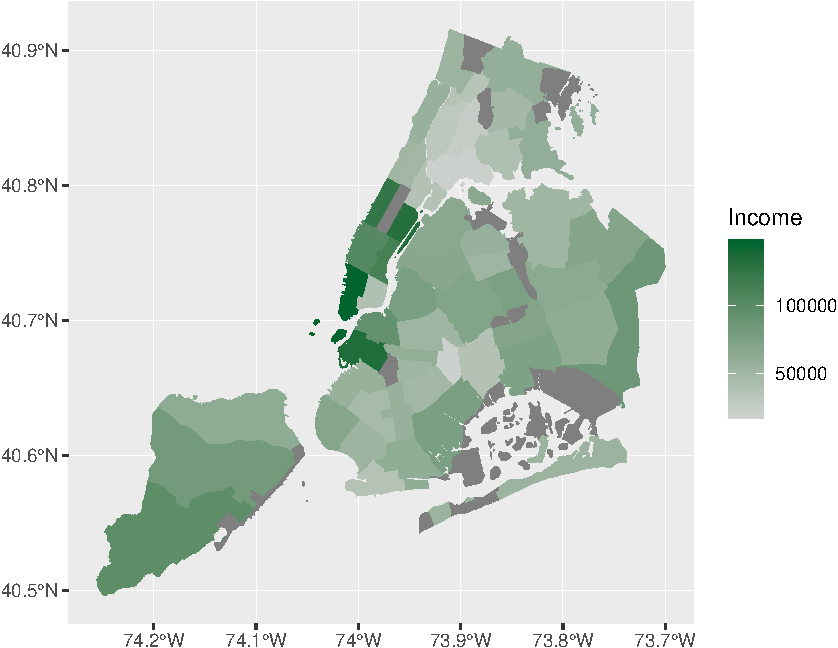
\includegraphics{KamalFinalPresentationPaper_files/figure-latex/unnamed-chunk-4-1} 

}

\caption{A choropleth map that indicates the income levels across New York City at the community district level}\label{fig:unnamed-chunk-4}
\end{figure}

\hypertarget{discussion}{%
\section{Discussion}\label{discussion}}

The sf package in R provides a multitude of ways for analysts to process geospatial data. This opens upon different avenues in the field of data science, especially designing predictive models of how income levels may continue to disperage across New York City. This would allow policymakers to truly have a more proactive approach to understand where exactly these disparities are occuring. For the user, there great deal of tools at their disposal with the sf package. They include converting non-spatial data frames to spatial data frames. For example, a dataset containing the Longitude and Latitude location of universities across New York City, but it is not a feature. That could be accomplished with the sf package.

\newpage

\hypertarget{references}{%
\section{References}\label{references}}

\begingroup
\setlength{\parindent}{-0.5in}
\setlength{\leftskip}{0.5in}

\hypertarget{refs}{}
\leavevmode\hypertarget{ref-keim2002information}{}%
Keim, D. A. (2002). Information visualization and visual data mining. \emph{IEEE Transactions on Visualization and Computer Graphics}, \emph{8}(1), 1--8.

\leavevmode\hypertarget{ref-R-sf}{}%
Pebesma, E. (2018). Simple Features for R: Standardized Support for Spatial Vector Data. \emph{The R Journal}. Retrieved from \url{https://journal.r-project.org/archive/2018/RJ-2018-009/index.html}

\leavevmode\hypertarget{ref-R-ggplot2}{}%
Wickham, H. (2016). \emph{Ggplot2: Elegant graphics for data analysis}. Springer-Verlag New York. Retrieved from \url{http://ggplot2.org}

\endgroup


\end{document}
